\subsubsection{Síncronos}

Nos contadores síncronos, todas as transições de estado ocorrem simultaneamente, pois todos os flip-flops são acionados pelo mesmo sinal de clock.

\begin{figure}[H]
   	\centering
   	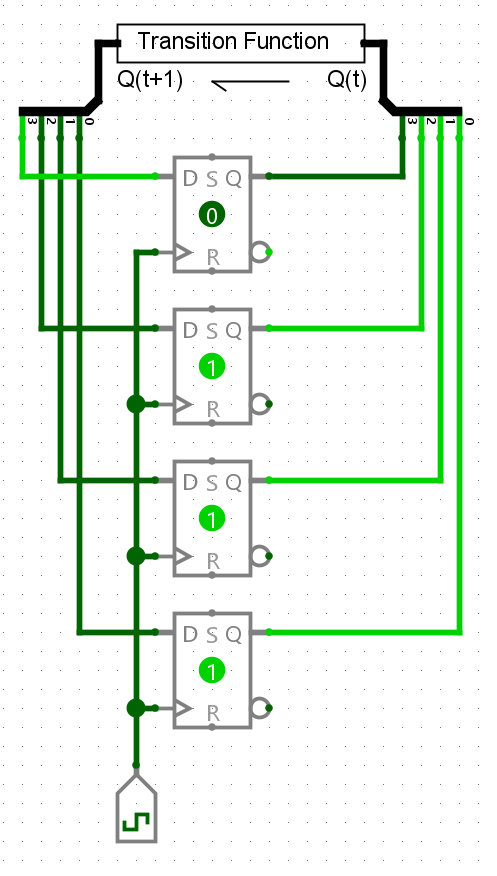
\includegraphics[width=0.31\linewidth]{images/sincrono-circuit.png}
  	 \caption{Circuito de um contador síncrono}
   	\label{fig:sincrono-circuit}
\end{figure}

Essa característica garante que a função de transição de estados seja aplicada de forma global e sincronizada, evitando atrasos acumulados entre bits.

Como consequência, contadores síncronos apresentam maior previsibilidade temporal e são mais adequados para aplicações que exigem precisão e confiabilidade.
